\documentclass[12pt]{article}

% General
\usepackage[round]{natbib}
\usepackage{setspace}
\usepackage{geometry}
\usepackage[section]{placeins}
\usepackage[hidelinks]{hyperref}
\usepackage{graphicx}
\usepackage{xcolor}
\usepackage{titlesec}
\usepackage[page]{appendix}
\usepackage{enumerate}

% Tables/Figures
\usepackage{lscape}
\usepackage{booktabs}
\usepackage{rotating}
\usepackage{multirow}
\usepackage{longtable}
\usepackage{caption}
\usepackage{subcaption}
\usepackage{float}
\usepackage{tabularx}
\usepackage{ragged2e}
\newcolumntype{Y}{>{\RaggedRight\arraybackslash}X}
\usepackage{pdflscape}
\usepackage{afterpage}

% Math
\usepackage{amsmath}
\usepackage{amssymb}
\usepackage{amsthm}
\usepackage{mathtools}
\usepackage{dsfont}

\usepackage{tikz}
\usetikzlibrary{bayesnet}

% \doublespacing
\onehalfspacing
% \singlespacing

% \numberwithin{equation}{section}

\geometry{paper=letterpaper, margin=1in}
\captionsetup{font=small}

% Code
\usepackage{textcomp}
\usepackage{sourcecodepro}
\usepackage{listings}
\definecolor{commentgrey}{gray}{0.45}
\definecolor{backgray}{gray}{0.96}
\lstset{
  basicstyle=\footnotesize\ttfamily, keywordstyle=\footnotesize,
  backgroundcolor=\color{backgray}, commentstyle=\color{commentgrey},
  frame=single, rulecolor=\color{backgray}, showstringspaces=false,
  breakatwhitespace=true, breaklines=true, upquote=true,
  numbers=left, numberstyle=\footnotesize\color{commentgrey}}

%%%%%%%%%%%%%%%%%%%%%%%%%%%%%%%%%%%%%%%%%%%%%%%%%%%%%%%%%%%%%%%%%%%%%%%%%%%%%%
% User-defined LaTeX commands
\DeclareMathOperator{\Var}{Var}
\DeclareMathOperator{\Cov}{Cov}
\DeclareMathOperator{\Corr}{Corr}
\DeclareMathOperator*{\argmax}{arg\,max}
\DeclareMathOperator*{\argmin}{arg\,min}
\DeclarePairedDelimiter{\abs}{\lvert}{\rvert}
\DeclarePairedDelimiter{\norm}{\lVert}{\rVert}
\newcommand*{\expp}[1]{\exp\left(#1\right)}
\newcommand*{\foralls}{\ \forall \ }
\newcommand*{\st}{\text{ s.t. }}
\newcommand*{\E}{\mathbb E}
\newcommand*{\R}{\mathbb R}
\newcommand*{\I}{\mathds{1}}
\newcommand*{\Prob}{\mathbb P}
\newcommand*{\convas}[1]{\xrightarrow{#1}}
\newcommand*{\conv}{\convas{}}
\newcommand*{\cond}{\;\ifnum\currentgrouptype=16 \middle\fi|\;}
\newcommand*{\defeq}{%
  \mathrel{\overset{\makebox[0pt]{\mbox{\normalfont\tiny\sffamily def}}}{=}}}
\newcommand*{\notorth}{\ensuremath{\perp\!\!\!\!\!\!\diagup\!\!\!\!\!\!\perp}}
\newcommand*{\orth}{\ensuremath{\perp\!\!\!\perp}}
\newcommand*{\evalat}{\,\big\rvert}
\newcommand*{\dif}{\,d}
\newcommand*{\difto}[1]{\,d^#1}
\newcommand*{\difbot}[1]{\frac{d}{d#1}}
\newcommand*{\partialbot}[1]{\frac{\partial}{\partial#1}}
\newcommand*{\m}[1]{\textbf{#1}}
\newcommand*{\bmath}[1]{\boldsymbol{#1}}

\newcommand*{\yestag}{\addtocounter{equation}{1}\tag{\theequation}}
\newcommand*{\notaligned}[1]{\noalign{$\displaystyle #1$}}
\newcommand*{\ttilde}{{\raise.17ex\hbox{$\scriptstyle\sim$}}}

\makeatletter
\newsavebox{\mybox}\newsavebox{\mysim}
\newcommand*{\distas}[1]{%
  \savebox{\mybox}{\hbox{\kern3pt$\scriptstyle#1$\kern3pt}}%
  \savebox{\mysim}{\hbox{$\sim$}}%
  \mathbin{\overset{#1}{\kern\z@\resizebox{\wd\mybox}{\ht\mysim}{$\sim$}}}%
}
\makeatother
\newcommand*{\dist}{\sim}
\newcommand*{\distiid}{\distas{\text{i.i.d}}}

\makeatletter
\def\moverlay{\mathpalette\mov@rlay}
\def\mov@rlay#1#2{\leavevmode\vtop{%
   \baselineskip\z@skip \lineskiplimit-\maxdimen
   \ialign{\hfil$\m@th#1##$\hfil\cr#2\crcr}}}
\newcommand*{\charfusion}[3][\mathord]{
  #1{\ifx#1\mathop\vphantom{#2}\fi\mathpalette\mov@rlay{#2\cr#3}}
  \ifx#1\mathop\expandafter\displaylimits\fi}
\makeatother
\newcommand*{\cupdot}{\charfusion[\mathbin]{\cup}{\cdot}}
\newcommand*{\bigcupdot}{\charfusion[\mathop]{\bigcup}{\cdot}}

\newcommand*{\mt}[1]{\text{\normalfont #1}}

\newtheorem{theorem}{Theorem}[section]
\newtheorem{theorem*}{Theorem}
\newtheorem{corollary}{Corollary}[section]
\newtheorem{proposition}{Proposition}[section]
\newtheorem{lemma}{Lemma}[section]

\theoremstyle{definition}
\newtheorem{definition}{Definition}[section]
\newtheorem{definition*}{Definition}
\newtheorem{example}{Example}[section]
\newtheorem*{properties}{Properties}

\newtheoremstyle{algodesc}{}{}{}{}{\bfseries}{.}{ }{}%
\theoremstyle{algodesc}
\newtheorem{algodesc}{Algorithm}
%%%%%%%%%%%%%%%%%%%%%%%%%%%%%%%%%%%%%%%%%%%%%%%%%%%%%%%%%%%%%%%%%%%%%%%%%%%%%%

\newcommand*{\colsquare}[3][-3.5pt]{\tikz[baseline=-0.5ex]\draw[#2, fill=#2] (0,#1) rectangle ++(#3,#3);}%
\definecolor{cmeet}{HTML}{B2DF8A}
\definecolor{cmideast}{HTML}{FDBF6F}
\definecolor{cstaff}{HTML}{A6CEE3}
\definecolor{cpolitics}{HTML}{33A02C}
\definecolor{cterror}{HTML}{E31A1C}
\definecolor{cforeign}{HTML}{FF7F00}
\definecolor{cpress}{HTML}{FB9A99}
\definecolor{chill}{HTML}{6A3D9A}
\definecolor{ccomm}{HTML}{1F78B4}


\begin{document}

\title{Exploring Hillary Clinton's Emails\thanks{STATS 601 final project. All of the code used to download, process, and analyze the data for this project is available at \url{https://github.com/lbybee/601_Final_Project} and has been open-sourced under the MIT license.}}
\author{
    Leland Bybee, Roger Fan, Ryan Vaughn
}
\date{April 22, 2016}

\maketitle


\section{Introduction}
From roughly 2008 to 2013, Hillary Clinton and some of her staff used a private family email server for most of he communication. This time period includes her tenure as U.S. Secretary of State, and has therefore become a controversial topic due to the possible security concerns of not using official government servers. Various investigations into the legality and appropriateness of the email server have been launched, and the issue has had/will potentiall have a large effect on Clinton's ongoing presidential campaign.

Due to several Freedom of Information Act (FOIA), the State Department has released the vast majority of the roughly 55,000 pages of emails to the public, leading to an unprecedented opportunity to explore the email usage of a major public figure.

Due to the size of the corpus, reading individual emails in the hope of discovering interesting characteristics is unrealistic. We therefore exploit statistical methods to break this vast analysis problem to a more manageable one, decreasing the scale so that we can more easily apply human and statistical analysis.

In order to tackle this problem, we use classical multi-dimensional scaling and spectral clustering in order to visualize and explore the corpus. We also use a statistical topic model, latent Dirichlet allocation (LDA), in order to identify and analyze the meanings and semantics. Finally, we use the LDA results and other metadata to examine how other covariates, such as email sender and time period sent, are related to the topic of an email.


\section{Data}
The State Department released the raw data in the form of roughly 30,000 pdfs of individual emails from the Clinton server.\footnote{Thanks to Ben Hamner and the Wall Street Journal for making the data processing code (\url{https://github.com/benhamner/hillary-clinton-emails}) and email pdfs (\url{http://graphics.wsj.com/hillary-clinton-email-documents/}) available, respectively.} We first process the pdfs to extract the raw text.\footnote{We used \texttt{pdftotext}, an open-source program used to extract text from pdf files.} From the raw email text, email headers and forward/response information are stripped, leaving only the subject line and body text.

All of our methods use a bag-of-words model, so from this raw data we construct a document term matrix containing vectors of word counts. Some standard data cleaning for text data is also performed, including the removal of punctuation and email addresses, word stemming (combining words with common roots, e.g. calling and called), and removing extremely common words (i.e. stop words) and extremely rare words (words that appear in less than 0.1\% of emails).

After this processing, we are left with a dataset of roughly 28,000 emails and a total vocabulary of over 3,000 words. Note that each word count vector is extremely sparse, so we need statistical methods that can apply in a sparse coordinate setting. Also, methods that can efficiently exploit this sparseness to reduce computation are preferred.


\section{Visualization}
Due to the large size and high dimensionality of the data, we must apply some dimensionality reduction in order to effectively visualize it. We therefore apply classical multi-dimensional scaling, which attempts to place each point in a much smaller dimension such that pairwise distances are preserved.

However, we expect standard Euclidean distance to poorly capture the actual relationships between vectors of word counts. In particular, Euclidean distance is affected by the total number of words, two emails with the exact same word distribution that differ in length could have a very large distance between them. In order to better capture pairwise relationships, we will use a distance metric based on the angles between vectors.

We define the cosine similarity between word frequency vectors $V$ and $W$ to be the cosine of the angle between the two vectors, calculated as
\begin{equation} \label{eq:cos_sim}
\cos(\phi) = \frac{\langle V, W \rangle}{\norm{V}\norm{W}}
\end{equation}
Since counts must be nonnegative, note that $\phi \leq \pi/2$. This implies that the cosine similarity is always between 0 and 1, with 0 corresponding to vectors that are multiples of each other and 1 corresponding to orthogonal vectors (i.e. no shared words). So we can define the cosine distance as
\begin{equation} \label{eq:cos_dist}
d(V, W) = 1 - \cos(\phi) = 1 - \frac{\langle V, W \rangle}{\norm{V}\norm{W}}
\end{equation}

Using this measure of distance, we can construct a distance matrix $D$ and apply MDS. The results for an 8,000 email subset are shown in Figure~\ref{fig:cluster}, plotted in both two and three dimensions. We can see several interesting patterns. The vast majority of emails (roughly 5,000) are contained in the main central grouping, with two large groupings that extend away. Besides these two ``arms,'' however, it is difficult to visually identify other significant structures.

\begin{figure}[htbp] \centering
  \begin{subfigure}[t]{.7\linewidth}
    \includegraphics[width=\linewidth]{../images/mds_2d_cluster.png}
    \caption{2 Dimensions} \label{fig:cluster:2d}
  \end{subfigure}
  \begin{subfigure}[t]{.7\linewidth}
    \includegraphics[width=\linewidth]{../images/mds_3d_cluster_1.png}
    \caption{3 Dimensions} \label{fig:cluster:3d}
  \end{subfigure}
  \caption{Visualization of a 8,000 email subset using classical multi-dimensional scaling and with coloring according to the results from spectral clustering. The similarity and distance metrics used for spectral clustering and MDS, respectively, are cosine similarity and distance as defined in Equations~\ref{eq:cos_sim} and~\ref{eq:cos_dist}.}
  \label{fig:cluster}
\end{figure}


\subsection{Spectral Clustering} \label{sec:spec_cluster}
In order to better identify structure that may exist in the data, we attempt to apply clustering methods. However, it is important to choose an appropriate clustering method due to the high dimensionality and sparse nature of the data. In particular, we expect centroid-based methods such as Gaussian mixture models and $k$-means clustering to perform poorly in this setting.

Spectral clustering, however, exploits the information contained in the pairwise distances (or, equivalently, the similarities) between points. By using pairwise distances, spectral clustering is particularly well-suited to finding clusters that may not necessarily be spherical or ellipsoidal and that may lie along lower-dimensional manifolds.

To actually apply spectral clustering, we first construct the pairwise similarity matrix $S$ using our cosine similarity as defined in Equation~\ref{eq:cos_sim}. We define the degree matrix $D$ to be a diagonal matrix with $D_{ii} = \sum_j S_{ij}$, and construct the symmatrix normalized Laplacian matrix as
\begin{equation} \label{eq:laplacian}
L = I - D^{-1/2} S D^{-1/2}
\end{equation}
Then the eigenvectors corresponding to the smallest $k$ eigenvalues of $L$ are computed and $k$-means clustering is performed on these eigenvectors.

Figure~\ref{fig:cluster} classifies each point according to the results of spectral clustering with $k$ clusters. We can see that many of the cluster correspond to  the visually identifiable structures, including clusters that correspond to each of the ``arms.''

By investigating the individual emails, we can also get a sense of what each cluster consists of. For instance, Clusters~2 and~4 consist of emails related to calls and communication. In this arm, those closer to the main central clump contain more conversation, while those farther out are much briefer and directly about the call (e.g. ``I'd like to call tomorrow.''). Cluster~3 consists entirely of ``minis,'' summaries of the days schedule sent to Clinton each morning. Emails from Cluster~5 are generally requests to print materials, while those from Cluster~6 are forwarded news articles.

In general, it seems that spectral clustering does a good job at identifying emails by their structure, but does not tell us much about the meaning of an email. We can tell that an email is regarding a call or is a news headline by what cluster it is in, but not what that call or headline is about. On a related note, it does not do a good job separating the ``regular'' emails. Over 5,000 of the 8,000 emails depicted fall into Clusters~1 or~8, which essentially consist of all the emails without specific identifiable structure. Ideally we would be able to further classify these emails according to subject matter, but clustering does not seem suited to this task.


\section{Topic Modeling}
To try and move beyond the limitations of spectral clustering and capture some of the content of the emails as well as structure, we next turn to latent Dirichlet allocation (LDA). LDA is a popular form of topic modeling that has historically been effective for identifying meaningful ``topics'' in text corpuses.  See Figure~\ref{fig:lda_graph} for a graphical representation of the model.  The model assumes that each document can be represented as a mixture of topics, and that each word is drawn based on the topic proportions in the corresponding document.  $\theta$ represents the topic proportion for each document and $\beta$ represents the topic weights for each word.  The model is estimated using variational Bayesian methods.

\begin{figure}
\centering
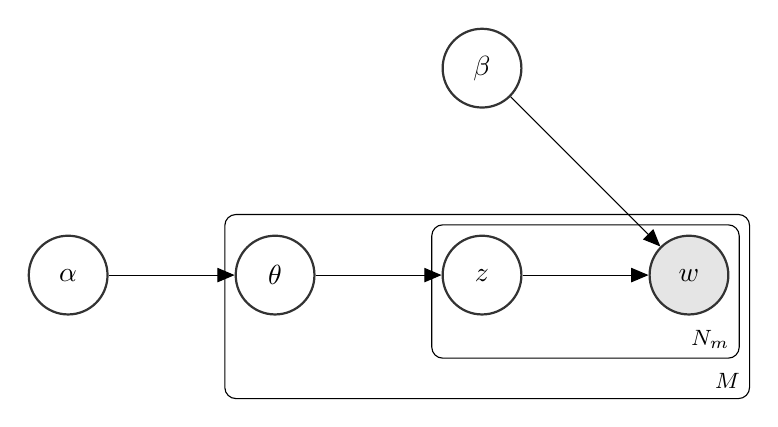
\begin{tikzpicture}[scale=1.0, every node/.style={transform shape}]
\tikzstyle{main}=[circle, minimum size = 10mm, thick, draw =black!80, node distance = 16mm]
\tikzstyle{connect}=[-latex, thick]
\tikzstyle{box}=[rectangle, draw=black!100]
  \node[main] (alpha) {$\alpha$};
  \node[main] (theta) [right=of alpha] {$\theta$};
  \node[main] (z) [right=of theta] {$z$};
  \node[main] (beta) [above=of z] {$\beta$};
  \node[main, fill=black!10] (w) [right=of z] {$w$};
  \edge {alpha} {theta};
  \edge {theta} {z};
  \edge {z,beta} {w};
  \plate {words} {(z)(w)} {$N_m$};
  \plate {docs} {(theta)(z)(w)(words.south east)(words.north west)} {$M$};
\end{tikzpicture}
\caption{LDA Graphical Representation}
\label{fig:lda_graph}
\end{figure}

The primary parameter that we need to specify for LDA is the number of topics. Since our ultimate goal is to find sensible topics that can be used to understand the email corpus, we initially turned to coherence measures, which attempt to quantify whether estimated topics would make sense to a human observer. In particular, we considered the UMass and UCI measures.\footnote{David Mimno, Hanna M. Wallach, Edmund Talley, Mirian Leenders, and Andrew McCallum. Optimizing Semantic Coherence in Topic Models. 2011.}\footnote{David Newman, Jey Han Lau, Karl Grieser, and Timothy Baldwin. Automatic Evaluation of Topic Coherence. 2010.}

% After estimating our final topic model we want to answer a series of questions concerning our resulting topics and the email corpus.  First, can we identify a sensible structure in our topics that captures the structure we see with spectral clustering?  Second, can we identify informative content topics that correspond to real world events?  Finally, can we say anything about the email senders based on the topics discussed?


\subsection{Interpreting Topics}
After choosing and estimating our topic model, the first task is to check whether we can actually find meaning in the resulting topics. If topics correspond to meaningful issues or structures then we can use these results to make useful observations about the data.

This ability to then perform ``human'' analysis on the results is one of the key features of LDA. Bringing human intuition to bear on a 28,000 email corpus is nearly impossible, but by condensing the data into a handful of topics LDA has allowed us to leverage our human understanding of semantics and meaning to analyze the data.

Interpretation is most easily done by examining the top words from each topics to find patterns and themes. Table~\ref{tab:top_words} shows the top 10 words for each of the 30 estimated topics. The LDA algorithm makes no attempt to interpret these meanings, but by viewing them there are several easily distinguishable patterns. For example, many of the top words in Topic~6 relate to Israel and Palestine. Not every topic is as well-identified as this, and some of the estimated topics are thematically weaker than others, but overall the topics seems to correspond very well to interpretable subjects.

\begin{table}[htb] \centering \scriptsize
\setlength{\tabcolsep}{4pt}
\begin{tabular}{cccccccccc}
  \toprule
  Topic 1 & Topic 2 & Topic 3 & Topic 4 & Topic 5   & Topic 6     & Topic 7  & Topic 8 & Topic 9   & Topic 10 \\
  \midrule
  call    & mistr   & know    & see     & state     & israel      & peopl    & think   & meet      & discuss  \\
  huma    & last    & just    & report  & benghazi  & isra        & world    & like    & reuters   & letter   \\
  abedin  & said    & want    & haiti   & inform    & peac        & power    & good    & follow    & draft    \\
  schedul & parti   & let     & news    & date      & palestinian & polit    & say     & update    & cdm      \\
  sheet   & david   & ask     & great   & subject   & netanyahu   & mani     & dont    & list      & note     \\
  request & prime   & come    & read    & agreement & east        & right    & look    & happi     & eam      \\
  speak   & deal    & tri     & media   & depart    & negoti      & can      & got     & monday    & secretar \\
  readout & leader  & sure    & event   & doc       & arab        & govern   & tell    & scshedule & question \\
  calls   & govern  & thx     & post    & hous      & state       & one      & thing   & set       & final    \\
  phone   & ireland & best    & connect & produc    & middl       & american & idea    & mtg       & brief    \\
  \bottomrule \\
  \toprule
  Topic 11   & Topic 12  & Topic 13 & Topic 14 & Topic 15 & Topic 16   & Topic 17   & Topic 18 & Topic 19 & Topic 20 \\
  \midrule
  democrat   & women     & new      & will     & make     & secretari  & senat      & libya    & iran     & time \\
  republican & clinton   & foreign  & work     & well     & depart     & bill       & secur    & syria    & press \\
  american   & right     & trip     & week     & take     & office     & vote       & travel   & nuclear  & hrc \\
  polit      & hillari   & told     & need     & way      & room       & health     & libyan   & syrian   & staff \\
  parti      & secretari & import   & next     & point    & state      & care       & iraq     & turkey   & dinner \\
  elect      & year      & agre     & also     & hope     & arriv      & pass       & embassi  & russia   & lona \\
  obama      & state     & high     & plan     & time     & rout       & hous       & attack   & regim    & ambassador \\
  percent    & human     & head     & start    & move     & privat     & john       & kill     & iranian  & close \\
  candid     & day       & later    & issu     & possibl  & offic      & committe   & march    & intern   & monica \\
  poll       & mani      & spoke    & keep     & one      & department & republican & august   & opposit  & remark \\
  \bottomrule \\
  \toprule
  Topic 21 & Topic 22 & Topic 23  & Topic 24 & Topic 25  & Topic 26 & Topic 27    & Topic 28 & Topic 29  & Topic 30 \\
  \midrule
  fyi      & said     & develop   & email    & presid    & china    & afghanistan & can      & statement & tomorrow \\
  print    & book     & state     & offic    & obama     & econom   & pakistan    & talk     & egypt     & today \\
  sid      & one      & support   & sent     & said      & year     & afghan      & get      & egyptian  & cheryl \\
  thank    & year     & global    & messag   & hous      & chines   & militari    & speech   & respond   & sullivan \\
  memo     & two      & program   & pleas    & white     & job      & general     & now      & announc   & jacob \\
  pls      & day      & effort    & may      & administr & million  & karzai      & back     & releas    & wil \\
  latest   & case     & intern    & check    & polici    & countri  & offici      & updat    & elect     & morn \\
  info     & famili   & work      & copi     & aid       & bank     & war         & send     & saudi     & jake \\
  intel    & school   & includ    & forward  & advis     & polici   & forc        & tonight  & reuter    & mill \\
  urgent   & court    & diplomaci & blair    & former    & economi  & nato        & soon     & presid    & confirm \\
  \bottomrule
\end{tabular}
\setlength{\tabcolsep}{6pt}

\caption{Topic Top Words}
\label{tab:top_words}
\end{table}

Another useful example is Topic~8, which does not seem to have any semantically meaningful words but primarily consists of ``common'' words like think, good, and tell. These ``structural'' topics illustrate one of the key advantages of the LDA model over spectral clustering. As we discussed in Section~\ref{sec:spec_cluster}, spectral clustering is only able to identify clusters based on the structure of emails, not their meaning. This is presumably because it primarily relies on the distribution of these ``common'' or ``structural'' words. By separating these types of words into separate topics, LDA is therefore able to better identify meaning in emails independent of their structure.


\subsection{Topic Categorization}
Looking through the word lists, we can roughly categorize the topics into overarching themes. This is obviously a subjective exercise, but is an example of how LDA can enable human, subjective analysis of the data. Table~\ref{tab:topic_cat} contains an example categorization.

\begin{table}[htb] \centering
\begin{tabular}{rcl}
  \toprule
  \colsquare{cterror}{10pt} & Terrorism & 5, 22 \\
  \colsquare{cmideast}{10pt} & Middle East & 6, 18, 19, 27, 29 \\
  \colsquare{cforeign}{10pt} & Foreign Policy & 2, 7, 13, 21, 23, 26 \\
  \colsquare{cpolitics}{10pt} & Politics & 11, 17, 25 \\
  \colsquare{cstaff}{10pt} & Staff & 16, 20 \\
  \colsquare{cpress}{10pt} & Press & 4 \\
  \colsquare{chill}{10pt} & Hillary & 12 \\
  \colsquare{cmeet}{10pt} & Meetings & 1, 9, 10, 24, 28, 30 \\
  \colsquare{ccomm}{10pt} & Common & 3, 8, 14, 15 \\
  \bottomrule
\end{tabular}
\caption{Topic Categorization}
\label{tab:topic_cat}
\end{table}

% The second thing that LDA gives is, for each email, a probability for every topic that the topic is included in the email.  Here, we will look at the relationships between topics and the frequencies that the topics are discussed.

% If we look at the entire data set, LDA will not give any topics probabilities of zero for any email, even if that topic realistically doesn't come up at all.  For example, here are the first six emails in the data set with the probabilities (in percent here) that each of the 30 topics is discussed in the email.

% PROBABILITY TABLE

% A few things jump out.  First, every topic is at least 1\% in each email (at least apparently in this grouping, but it's this way throughout the entire set).  Second, some emails aren't about very much at all.  Email 1 has 3\% for everything and 9\% for topic 3, which was a common topic.  Contrast this with email 2, which has a low \% for every topic except 18, 19, 21, 25.  We could hypothesize that this email is about the Middle East, Foreign Policy, and Domestic Politics.  We could, of course, do this kind of procedure with email after email, but with 28,000 emails we need a way to get meaning from the whole group.

% Before analyzing, we will remove the percentages for the common topics for each email, since we can realistically say that no email is about a topic with ``can'', ``also'', ``will'', etc., as the key words.  Next, we will zero any topic for each email that has less than 5\%.  The reason for this is the same as the logic in the above paragraph.  For email 2, we would naturally seek the topics with the higher percentages and ignore the rest.  After this we will rescale the percentages.

In the LDA model, a document is a probability distribution over the available topics. We also estimate these topic proportions for each email. To get an idea of the most common topics, we identify the ``primary'' topic in each email.\footnote{To identify primary topics, we ignore ``common'' topics as identified in Table~\ref{tab:topic_cat}. Then for each email we identify the highest percentage topic as the ``primary'' topic.} Table~\ref{tab:topic_freq} ranks the topics in terms of how frequently they are the primary topic.

\begin{table}[htb] \centering
\setlength{\tabcolsep}{1pt}
\begin{tabular}{cccccccccccccccccccccccccc}
  \toprule
  \colsquare[-3pt]{cforeign}{15pt} &
  \colsquare[-3pt]{cmeet}{15pt} &
  \colsquare[-3pt]{cmeet}{15pt} &
  \colsquare[-3pt]{cmeet}{15pt} &
  \colsquare[-3pt]{cmeet}{15pt} &
  \colsquare[-3pt]{cmeet}{15pt} &
  \colsquare[-3pt]{cpress}{15pt} &
  \colsquare[-3pt]{cmeet}{15pt} &
  \colsquare[-3pt]{cmideast}{15pt} &
  \colsquare[-3pt]{cmideast}{15pt} &
  \colsquare[-3pt]{cstaff}{15pt} &
  \colsquare[-3pt]{chill}{15pt} &
  \colsquare[-3pt]{cstaff}{15pt} &
  \colsquare[-3pt]{cpolitics}{15pt} &
  \colsquare[-3pt]{cforeign}{15pt} &
  \colsquare[-3pt]{cmideast}{15pt} &
  \colsquare[-3pt]{cforeign}{15pt} &
  \colsquare[-3pt]{cmideast}{15pt} &
  \colsquare[-3pt]{cterror}{15pt} &
  \colsquare[-3pt]{cmideast}{15pt} &
  \colsquare[-3pt]{cforeign}{15pt} &
  \colsquare[-3pt]{cpolitics}{15pt} &
  \colsquare[-3pt]{cforeign}{15pt} &
  \colsquare[-3pt]{cforeign}{15pt} &
  \colsquare[-3pt]{cpolitics}{15pt} &
  \colsquare[-3pt]{cterror}{15pt} \\
  21 & 1 & 28 & 30 & 10 & 9 & 4 & 24 & 18 & 29 & 16 & 12 & 20 &
  17 & 13 & 19 & 23 & 27 & 22 & 6 & 2 & 25 & 26 & 7 & 11 & 5 \\
  \midrule
  \multicolumn{13}{l}{Most Frequent} & \multicolumn{13}{r}{Least Frequent} \\
  \bottomrule
\end{tabular}
\setlength{\tabcolsep}{6pt}
\caption{Primary Topic Frequency}
\label{tab:topic_freq}
\end{table}

There are several interesting observations we can make from Tabels~\ref{tab:topic_cat} and~\ref{tab:topic_freq}. An easy one is that many of these emails are about meetings and similar issues. This not only makes sense because of Clinton's position as Secretary of State, where she presumably spends a large amount of time in meetings or briefings, but also because these shorter, administrative emails create high volume and are constantly being sent.

We can also observe that relatively few of the topics are about domestic issues such as health care, the economy, or education. Again, this matches what we would expect given that Clinton's position of Secretary of State means that she primarily deals with foreign affairs, which many of the topics are related to.

% Speaking of foreign affairs, the topic frequency for the purple above is much less than we might expect, except for 21.  This could be perceived as a bit unexpected from the Secretary of State.  This generalization might be unfair, however, because other specific foreign affair topics like 18 and 29 are higher and are about, for example, the Middle East.


\subsection{Topic Analysis}
We can also look into specific topics in more detail to see what they consist of and how they might correspond to real-world events. Table~\ref{tab:content_topics} shows the top 10 words for six topics that are all examples of content topics. In particular, these topics correspond to specific politically significant events or issues. For instance, the Libya topic seems to capture discussion about the Benghazi scandal as well the collapse of Gaddafi's administration.

\begin{table}[h] \centering
\begin{tabular}{cccccc}
  \toprule
  Topic 6     & Topic 11   & Topic 18 & Topic 27    & Topic 23  & Topic 25 \\
  Israel      & Elections  & Libya    & Afghanistan & Int. Dev. & Obama \\
  \midrule
  israel      & democrat   & libya    & afghanistan & develop   & presid \\
  isra        & republican & secur    & pakistan    & state     & obama \\
  peace       & american   & travel   & afghan      & support   & said \\
  palestinian & polit      & libyan   & militari    & global    & hous \\
  netanyahu   & parti      & iraq     & general     & program   & white \\
  east        & elect      & embassi  & karzai      & effort    & administr \\
  negoti      & obama      & attack   & offici      & intern    & polici \\
  arab        & percent    & kill     & war         & work      & aid \\
  state       & candid     & march    & forc        & includ    & advis \\
  \bottomrule
\end{tabular}
\caption{Some interesting content topics}
\label{tab:content_topics}
\end{table}

The model seems to effectively identify words that human observers would associate with these events. Topic~11 picks up on both of the primary political parties in the United States as well as other words associated with elections, such as politics, percent, and candidate. Similarly, the Topic~23 identifies words that associated with international development, including develop, support, and global.

Given that we have time stamps foe each email, we can also examine how prevalent each topic is over time. Figure~\ref{fig:topic_time_plots} shows the mean monthly topic proportion for each of the topics in Table~\ref{tab:content_topics}.

\begin{figure}[htb]
\centering
\begin{subfigure}[Israel]{.30\linewidth}
    \includegraphics[width=\linewidth]{../images/time_plot6.pdf}
    \caption{Israel} \label{fig:t1}
\end{subfigure}
\begin{subfigure}[Elections]{.30\linewidth}
    \includegraphics[width=\linewidth]{../images/time_plot11.pdf}
    \caption{Elections} \label{fig:t2}
\end{subfigure}
\begin{subfigure}[Libya]{.30\linewidth}
    \includegraphics[width=\linewidth]{../images/time_plot18.pdf}
    \caption{Libya} \label{fig:t3}
\end{subfigure}
\begin{subfigure}[Afghanistan]{.30\linewidth}
    \includegraphics[width=\linewidth]{../images/time_plot27.pdf}
    \caption{Afghanistan} \label{fig:t4}
\end{subfigure}
\begin{subfigure}[Int. Dev.]{.30\linewidth}
    \includegraphics[width=\linewidth]{../images/time_plot23.pdf}
    \caption{Int. Dev.} \label{fig:t5}
\end{subfigure}
\begin{subfigure}[Obama]{.30\linewidth}
    \includegraphics[width=\linewidth]{../images/time_plot25.pdf}
    \caption{Obama} \label{fig:t6}
\end{subfigure}
\caption{Average monthly topic proportions.}
\label{fig:topic_time_plots}
\end{figure}

We can see that our topics seem to be correlated with the expected real-world events. The Israel topic's first peak corresponds to the July 26th, 2010 joint Israeli and Romanian helicopter disaster, while the second peak corresponds to the September 9th, 2011 attack on the Israel embassy in Egypt. Similarly, for the election topic each of the peaks corresponds to a U.S. election. Looking at the Libya topic, the first peak corresponds to the fall of Gaddafi's adminstration in October of 2011, while the second peak corresponds to the Benghazi attack on September 11th, 2012. These kinds of patterns over time are interesting to verify, and could also be used to identify the prevalent topics of discussion for times when there are not obvious world events driving discussion.\footnote{These monthly topic proportion plots for all our estimated topics are available at \url{https://github.com/lbybee/601_Final_Project/tree/master/images}.}


\section{Email Sender Prediction}
Finally, we want to consider whether we can say anything interesting about the senders based on our topic model. In total 395 unique senders exist in our email corpus, however, only 14 senders sent more than 100 emails. We focus on this subset of 14 senders for the remainder of our analysis. This leaves us with a corpus of 25809 emails. We use the topic proportions from the model estimated on the full corpus for this subset.

\begin{table}[htb] \centering \scriptsize
\begin{tabular}{cccccc}
  \toprule
  Israel & Elections & Libya & Afghanistan & Int. Dev. & Obama \\
  \midrule
  Sidney Blumenthal & SB & Huma Abedin & Judith McHale & JM & SB \\
  (SB) & & (HA) & (JM) & & \\
  \noalign{\vskip 5mm}
  HA & Philippe Reines & Wendy Sherman & HA & Melanne Verveer & PR \\
  & (PR) & (WS) & & (MV) & \\
  \noalign{\vskip 5mm}
  Jake Sullivan & JM & JS & MV & Anne-Marie & Cherly Mills \\
  (JS) & & & & Slaughter (AMS) & (CM)\\
  \noalign{\vskip 5mm}
  AMS & CM & Monica Hanley & JS & CM & HA \\
  & & (MH) & & & \\
  \noalign{\vskip 5mm}
  Hillary Clinton & HA & SB & Richard Verma & JS & HC \\
  (HC) & & & (RV) & & \\
  \bottomrule
\end{tabular}
\caption{Primary senders for interesting topics}
\label{tab:top_senders}
\end{table}

See Table~\ref{tab:top_senders} for a ranking of the 14 senders for the subset of content topics explored above. This table presents the top five senders for each of the topics based on the average topic proportion for each sender. The sorting that we get back seems to fit with a human understanding of each of the senders, Sidney Blumenthal, who appears to be most associated with the Israel, Election and Obama topics is a long standing advisor to the Clinton family who has written extensively on US politics as well as foreign policy. Similarly, Huma Abedin, who is most associated with Libya was a key figure during the Benghazi hearings and was generally strongly associated with foreign policy, particularlly in the Middle East while Hillary Clinton's Deputy Chief of Staff. Finally, Judith McHale, who is most associated with the Afghanistan and international development topic was Under Secretary of State for Public Diplomacy and Public Affairs during the early portion of the email corpus under Hillary. She also has been strongly associated with a number of philanthropic efforts. It may be interesting to note that Hillary does not appear to be strongly associated with many of our subset of content topics. This pattern persists through the remainder of the content topics, in general, Hillary does not appear to send many emails strongly associated with most of the content topics.


\subsection{Multinomial Logistic Regression}
While the above results do give some sense of which senders are most associated with which topics, we next want to formalize this approach and get more general results that can more easily show us which senders are most related to each topic. To approach this problem we turn to multinomial logistic regression as a solution. Multinomial logistic regression generalizes the logistic regression approach to the case with more labels than two. The probability that the $j$th label is assigned to the $i$th email is,

\begin{equation} \label{eq:smax}
p(y_i = j | x_i, \boldsymbol{\beta}) = \frac{\exp\{\beta_j^Tx_i\}}{\sum_{1\leq k\leq K} \exp\{\beta_k^Tx_i\}}
\end{equation}

This produces a $P \times K$ matrix of coefficients, $\boldsymbol{\beta}$, corresponding to how strongly related each of the $K$ variables of interest are related to each of the $P$ labels.

For our particular case we estimate a model using the $30$ topics as our explanatory variables and the $14$ senders as our labels. We use a training subset of 23229 emails and their corresponding topic proportions to train our model and a subset of 2580 emails for testing. See table \ref{tab:mlr_success} for the success rate for our testing data. Overall the model appears to perform well, correctly identifying roughly 30\% of the senders correctly. For Hillary we correctly identify 74\% of the emails.

\begin{table}[htb] \centering
\begin{tabular}{ccc}
  \toprule
  Source               & Success Rate & Testing Observations \\
  \midrule
  Hillary Clinton      & 0.74         & 849 \\
  Philippe Reines      & 0.06         & 34 \\
  Claire Coleman       & 0.52         & 27 \\
  Lauren Jiloty        & 0.42         & 71 \\
  Huma Abedin          & 0.36         & 376 \\
  Jake Sullivan        & 0.23         & 410 \\
  Sidney Blumenthal    & 0.29         & 87 \\
  Cherly Mills         & 0.31         & 491 \\
  Anne-Marie Slaughter & 0.36         & 42 \\
  Monica Hanley        & 0.09         & 53 \\
  Judith McHale        & 0.25         & 28 \\
  Robert Russo         & 0.00         & 10 \\
  Richard Verma        & 0.26         & 19 \\
  Wendy Sherman        & 0.08         & 12 \\
  Melanne Verveer      & 0.30         & 30 \\
  Lona Valmoro         & 0.34         & 41 \\
  \bottomrule
\end{tabular}
\caption{Multinomial logistic regression test results.}
\label{tab:mlr_success}
\end{table}

To relate these results back to our earlier analysis we want to look at the coefficients for the multinomial logistic regression model as this should give us a sense of how strongly each sender is associated with the different topics. See Figure~\ref{fig:coefficients} for a heatmap of the resulting coefficient matrix.\footnote{Note that the coefficients are standardized and then thresholded at $\pm2$ for illustrative purposes.}

The results we see here all us to tell a story about the email senders that corresponds to our intution based on each of the sender's backgrounds. Sidney Blumenthal is strongly associated with the Middle East, foreign policy and general politics topics. He doesn't have much to say about Hillary or her significance to the press and generally doesn't talk muhc about meetings. Huma Abedin and Jake Sullivan provide advice on the Middle East and foreign policy. Judith McHale focuses her emails on foreign policy and handling press issues. While all this is going on Hillary spends most of her time discussing meetings.

In general the story that emerges is that while Hillary does not say much herself about world events, she has surrounded herself with a set of advisors who are more than willing to say a great deal about the content topics. She then spends most of her time on email coordinating meetings, telling people to print emails and generally coordinating the information gathered from her advisors.

\begin{figure}[htb] \centering
  \includegraphics[width=0.95\linewidth]{../images/coefficients.pdf}
  \caption{Standardized coefficients from a multinomial logistic regression of email sender on LDA topic proportions.}
  \label{fig:coefficients}
\end{figure}


\section{Conclusion}
We have presented a series of results to attempt to make a large corpus of emails that would be difficult to parse manually approachable to the human user. We have been able to identify general structures in the email corpus using both spectral clustering and LDA. For LDA we find that we can seperate out content topics from structural topics and that the topics we get back are sensible and align with what we would expect in the real world. Additionally, we find that we can say something interesting about the senders for our email corpus.

There are many ways that this work could be expanded, and our work should be considered explorartory and a starting place more than anything else. While we begin to dive into some possible extensions when we discuss senders this idea could easily be taken further. Information on recievers, while not as clean as sender information could also be incorporated. This could allows us to build a better model of interactions within the email corpus. Additionally, variables beyond just the topic proportions could be incorporated into our model, one clear example of this is a time spline variable to account for the possibility that different senders are more important for different topics over time.

Overall, we have tried to tell a story about the Hillary email corpus. We have only scratched the surface of our understanding of this corpus but we believe that we have layed out a good set of tools and a strong approach to move forward.

\end{document}
